%!Mode:: "TeX:UTF-8"

\section{Linux Bonding}


Linux的多网卡绑定技术是在网卡驱动程序之上、数据链路层之下实现的一个虚拟层,它将多个网卡虚拟成一块虚拟网卡,所以多网卡绑定驱动程序实际上是一种中间驱动程序,是基本驱动程序与网络协议栈之间的接口。


\begin{figure}
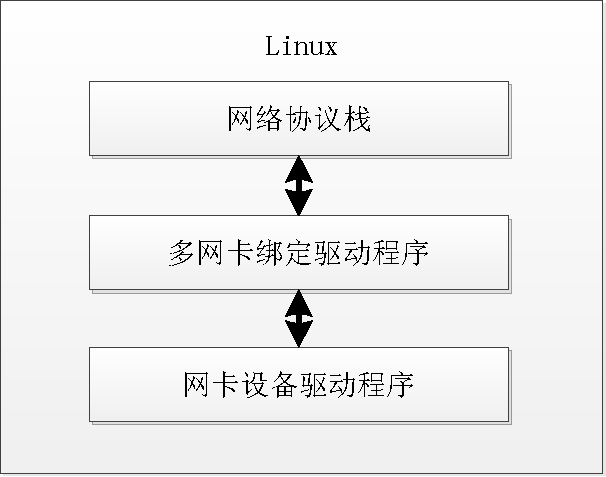
\includegraphics[keepaspectratio,width=0.4\paperwidth]{Pictures/LinuxBondingDriver.pdf} 
\caption{Linux多网卡绑定原理图}
 \label{fig:LinuxBondingDriver}
\end{figure}



目前Linux现有的多网卡绑定驱动共有七种传输模式(算法),依次是:轮转模式、热备份模式、异或模式、广播模式、动态链路聚合模式、自适应传输负载平衡模式、自适应负载平衡模式。\textbf{其中最常用的是模式0、1和6。}

在轮转算法中所有优先级相同的网卡设备维持在一个循环队列中,队列的每个节点(网卡)具有相同的地位,多网卡绑定驱动在这些网卡设备中顺序轮流选择,队列中所有的成员公平分享所有的传输任务。轮转算法的适用面最广,轮转模式适用于绑定驱动中所有节点的处理能力和性能均相同的情况,如适用相同类型的网卡。它的算法思想虽然很简单,但传输能力和传输效率是最好的,不过需要交换机支持,如果交换机未配置链路聚合,则会发生MAC地址表的动荡,在配置了链路聚合后不会出现,发出数据包的MAC为虚拟网卡Bond0的MAC,限制了它的一些应用场合。

模式1的热备份算法可以用来提高服务器的高可用性,在主网卡失效的情况下,备用网卡可以接替主网卡继续工作,但是网卡的利用率只有1/N,效率较低。
    
模式6的平衡负载模式,有自动备援,无需交换机特殊配置,即可实现负载均衡,它们的动态负载均衡方式可以根据绑定设备中网卡的负载状态来动态的分配传输任务,主要适用于服务器拥有四块及四块以上网卡的情况。
